\documentclass[12pt]{article}
\usepackage{amssymb,amsmath,bm,graphicx}
\usepackage{float}

\pagestyle{myheadings}

\begin{document}
\thispagestyle{plain}
\begin{center}
{\Large \bf Project}

\medskip
{\bf Due on August 7th, 2022}
\end{center}
\noindent
Consider the following ordinary
differential equation for $u$:
\begin{equation}
\label{de}
-u''(x)+\pi^2 \cos^2(\pi x) u(x) = f(x)\ \ \ x \in [0,1]
\end{equation}
with boundary conditions:
\begin{eqnarray}
\label{bc}
u(0) &=& 0, \nonumber \\
u(1) &=& 0.
\end{eqnarray}
\begin{description}
\item[1.] Consider
$f(x) = \pi^2 \sin(\pi x) \cosh(\sin (\pi x) )$,
and check that the function $u(x) = \sinh ( \sin (\pi x) )$ is the
solution to the
boundary value problem (BVP) (\ref{de})+(\ref{bc}).

\item[\textbf{solution.}]
Consider $u(x)=\sinh(sin (\pi x) )$,we have:
\begin{eqnarray}
    u(0)=\sinh(0)=0,\nonumber\\
    u(1)=\sinh(0)=0.
\end{eqnarray}
and
\begin{equation}
    u^{'}(x)=\cosh(\sin (\pi x) )\pi \cos (\pi x)
\end{equation}
\begin{equation}
    u^{''}(x)=\pi^{2}\sinh(\sin (\pi x) )\pi \cos^{2} (\pi x)-\pi^{2}\cosh(\sinh(\pi x))\sin(\pi x)
\end{equation}
so
% \begin{equation}
% \begin{aligned}
%     &-u^{''}+\pi^2 \cos^2(\pi x) \\
%     =& \pi^2sin(\pi x)\cosh(\sinh(\pi x))-\pi^{2}\sinh(\sin (\pi x) )\pi \cos^{2} (\pi x)\\
%     &+\pi^2 \cos^2(\pi x)\sinh(\sin (\pi x))\\
%     =& \pi^2 \sin(\pi x) \cosh(\sin (\pi x) )
%     =& f(x)
% \end{aligned}
% \end{equation}

\begin{equation}
    \begin{aligned}
    -& u^{\prime \prime}+\pi^{2} \cos ^{2}(\pi x)  \\
    =& \pi^{2} \sin (\pi x) \cosh (\sinh (\pi x))-\pi^{2} \sinh (\sin (\pi x)) \pi \cos ^{2}(\pi x)  \\
    &+\pi^{2} \cos ^{2}(\pi x) \sinh (\sin (\pi x))  \\
    =& \pi^{2} \sin (\pi x) \cosh (\sin (\pi x))=f(x)
    \end{aligned}
    \end{equation}


\item[2.] We want to solve this BVP
numerically. We begin by
discretizing the interval $[0,1]$. For this, consider the gridpoints:
\begin{equation}
x_i = i h,\ \ i=0,1,\dots,n+1,\  \ h=\frac{1}{n+1}.
\end{equation}
Note that $h_i = x_{i+1}-x_i = h$ for all $i$.  Now we approximate the
second derivative. Show that if $g$ has four
continuous derivatives, then
\begin{equation}
\label{approx}
\frac{g_{i+1}-2g_i+g_{i-1}}{h^2} = g''_i + O(h^2),
\end{equation}
where $g_i = g(x_i)$.


\item[\textbf{solution.}]
According to the Taylor expansion,we have the following equations:
\begin{eqnarray}
    \label{f}
    g_{i+1}-g_{i} &=& g_{i}^{'}h+\frac{1}{2!}g_{i}^{''}h^{2}+\frac{1}{3!}g_{i}^{'''}h^{3}+O(h^4)  \\
    \label{g}
    g_{i-1}-g_{i} &=& -g_{i}^{'}h+\frac{1}{2!}g_{i}^{''}h^{2}-\frac{1}{3!}g_{i}^{'''}h^{3}+O(h^4)
\end{eqnarray}
(\ref{f})+(\ref{g})
\begin{equation}
    \label{h}
    g_{i+1}-2g_i+g_{i-1} = h^2g_i^{''}+O(h^4)
\end{equation}
that is:
\begin{equation}
    \label{i}
    \frac{g_{i+1}-2g_i+g_{i-1}}{h^2}=g_i^{''}+O(h^2)
    \end{equation}

\item[3.] Consider now the linear system of equations
\begin{equation}
\label{system}
- \frac{g_{i+1}-2g_i+g_{i-1}}{h^2}+\pi^2 \cos^2 (\pi x_i )\, g_i = f(x_i)\
\ i=1,2,\dots,n.
\end{equation}
Show that this can be rewritten in matrix form as
\[
\bm{ A} \cdot \bm{ g} = \bm{ f},
\]
where $\bm{ g} = (g_1,\dots,g_{n})^T$,
$\bm{ f} = (f_1,\dots,f_{n})^T$, and the matrix $\bm{ A}$ is
tridiagonal, with entries:
\begin{equation}
a_{i,j} = \left \lbrace \begin{array}{cr} -\frac{1}{h^2}& |i-j|=1, \\
	\frac{2}{h^2} + \pi^2 \cos^2(\pi x_i) & i=j, \\
0& Otherwise. \end{array}
\right .
\end{equation}

\item[\textbf{solution.}]
\begin{equation}
    A=
\begin{pmatrix}
    \frac{2}{h^2} + \pi^2 \cos^2(\pi x_1) & -\frac{1}{h^2} & &  \\
    -\frac{1}{h^2} & \frac{2}{h^2} + \pi^2 \cos^2(\pi x_2) & -\frac{1}{h^2} & \\
     &  & \ddots & & \\
     & & -\frac{1}{h^2} & \frac{2}{h^2} + \pi^2 \cos^2(\pi x_n)
\end{pmatrix}
\end{equation}
so according to the 
\begin{equation}
    \begin{aligned}
    -&\frac{1}{h^2}g_{i+1}+(\frac{2}{h^2} + \pi^2 \cos^2(\pi x_2))\times g_i-\frac{1}{h^2}g_{i-1}\\
    =&- \frac{g_{i+1}-2g_i+g_{i-1}}{h^2}+\pi^2 \cos^2 (\pi x_i )\, g_i = f(x_i)\ 
    \ i=1,2,\dots,n.
    \end{aligned}
\end{equation}
and
\begin{equation}
    g_0=g_n=0
\end{equation}


\item[4.] Show that Scheme  \eqref{system} is second-order accurate.
\item[\textbf{solution.}]
If $g(x)$ is the exact solution to the problem(\ref{de})+(\ref{bc}),
that is:
\begin{equation}
    -g''(x)+\pi^2 \cos^2(\pi x) g(x) = f(x)
\end{equation}
according to the Taylor expansion
\begin{equation}
- \frac{g_{i+1}-2g_i+g_{i-1}}{h^2}+\pi^2 \cos^2 (\pi x_i )+O(h^2)=f(x_i)
\end{equation}
compaired with \eqref{system},the local truncation error of \eqref{system} is $O(h^2)$


\item[5.] Solve the system of equations
(\ref{system}). Use the following values: $n=10$, $20$, $40$, $80$, $160$, $320$.
For each $h=1/(n+1)$, compute the error
\begin{equation}
e(h) = \sup_{1\le i \le n} |g_i - u(x_i)|
\end{equation}
and do a log-log plot of $e(h)$, that is, plot $\log(e(h))$ as a
function of $\log(h)$. Show, using this plot, that $e(h) = O(h^2)$,
consistent with \textbf{4}.
\item[\textbf{solution.}]
\begin{figure}[H]
    \centering
    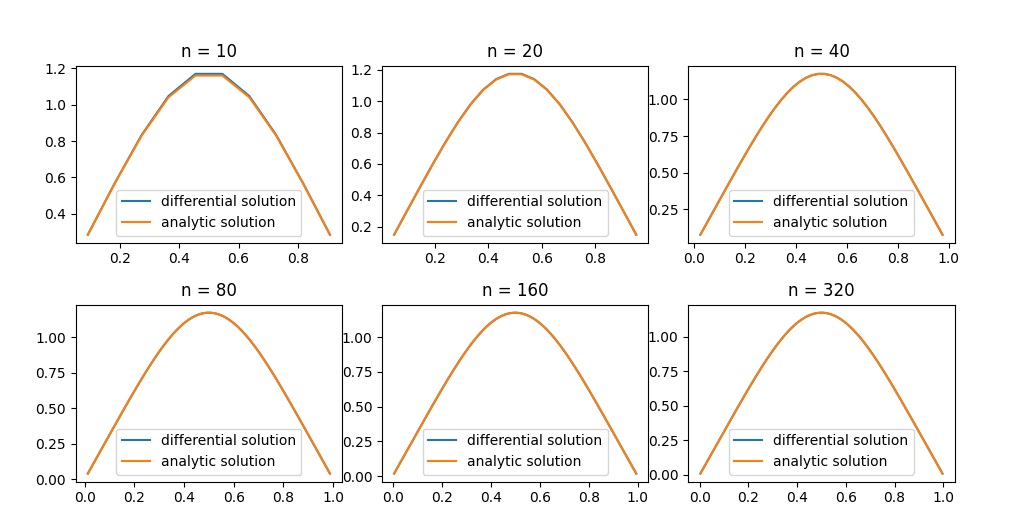
\includegraphics[width=\textwidth]{gra/solution5.png}
    \caption{solution}
\end{figure}

\begin{figure}[H]
    \centering
    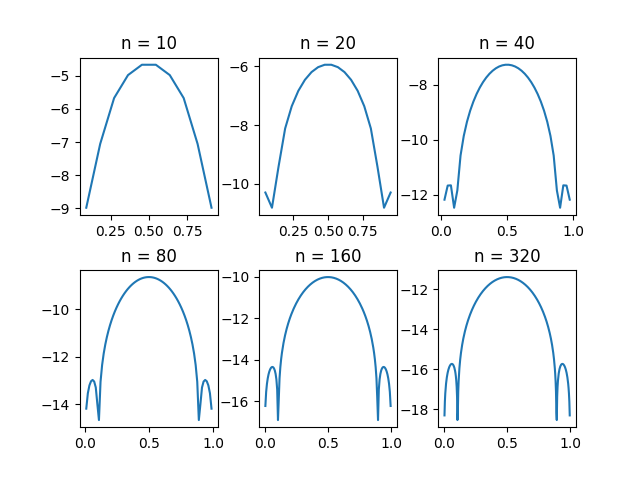
\includegraphics[width=\textwidth]{gra/error5.png}
    \caption{error}
\end{figure}


\item[6.] Consider a neural network solution in the following form
\begin{equation}
u_{\mathrm{NN}}(x) = x(1-x)\left(\sum_{i=1}^{n-1} u_i \sin(w_i x + b_i) \right),
\end{equation}
which satisfies the boundary condition. The loss function in the least-squares sense is
\begin{equation}
\sum_{i=1}^{n-1} \left( -u_{\mathrm{NN}}''(x_i)+\pi^2 \cos^2(\pi x_i) u_{\mathrm{NN}}(x_i) - f(x_i) \right)^2.
\end{equation}
Use Adam or stochastic gradient descent method to find the optimal set of parameters $\{u_i, w_i, b_i\}_{i=1}^{n-1}$.
Use the following values: $n=10$, $20$, $40$, $80$, $160$, $320$. For each $n$, compute the error
\begin{equation}
e(n) = \sup_{1\le i \le n} |u_{\mathrm{NN}}(x_i) - u(x_i)|.
\end{equation}
What is the conclusion we can draw for the neural network solution? Compare this result with that of the second-order difference scheme.
\end{description}

Send your project with your name, your student ID to jingrunchen@ustc.edu.cn.

\end{document}